\documentclass[10pt]{article}

\usepackage[letterpaper, margin=1in]{geometry}
\usepackage{parskip}
\usepackage{graphicx}
\usepackage{authblk}
\usepackage{amsmath}
\usepackage{braket}

\title{Motor Learning of the Optokinetic Response}

\author[1]{Daniel Popp}
\author[2]{Marcelo Beramendi Cabellero}
\affil[1]{Report Author}
\affil[2]{Project Partner}

\begin{document}

\maketitle

\section{Introduction}

In this project, we sought to replicate and expand on the results of Yamazaki, et. al. in their 2015 paper, ``Modeling Memory Consolidation During Posttraining
Periods in Cerebellovestibular Learning." In their paper, Yamazaki et. al. create a computational model of motor learning of the optokinetic response. Through running various simulations, they demonstrate that both long-term potentiation at mossy fiber-vestibular nuclear neuron synapses and long-term depression at parallel fiber-Purkinje cell synapses play important roles in motor learning, providing evidence to reconcile two competing hypotheses regarding the mechanisms of motor learning \cite{yamazaki2015modeling}.

\subsection{Optokinetic Response}

The optokinetic response is a reflexive eye movement in response to movement of the visual field. As we move through the environment, a series of small, rapid eye movements allows for the production of a stable image of the environment, critical for any sort of functioning.

The optokinetic response can be studied in vitro by measuring eye movements in response to a moving visual field, often simulated in manners such as the movement of stripes across a screen. The proportion to which the movements of the eye matches the movement of the visual field is called OKR gain. This gives a concrete measurement to study how the optokinetic response improves with training.

\subsection{The Cerebellar Network}

The neural underpinnings of the optokinetic response lie in the cerebellum. A simplified version of the network can be described as follows:

The cerebellum receives input via signals from mossy fibers (MFs) and climbing fibers (CFs). Mossy fibers carry sensory information to the cerebellum about the state of the body and the environment, and the intended movement of the body \cite{knierim2014information}. In generating the optokinetic response, this would include information about the position of the target the eyes are following, and the position and movement of the eyes themselves. These mossy fibers provide excitatory inputs to the granule cells (GCs) of the cerebellum. These granule cells have long unmyelinated axons with parallel branches, dubbed the parallel fibers (PFs), which carry excitatory input to molecular-layer interneurons (MLIs) such as stellate and basket cells, and Purkinje cells (PCs). The MLIs convert the excitatory input from the GCs to an inhibitory input to the PCs. PCs additionally receive excitatory input from climbing fibers, the other source of input to the cerebellum. Purkinje cells (PCs) are the sole output path from the cerebellum, providing inhibitory signals to the vestibular nuclear neurons (VNs) in the vestibular nuclei \cite{sillitoe2012cerebellum}. The VNs also receive excitatory input from the MFs. Finally, the VNs carry signals back to the eyes to control their movement \cite{yamazaki2015modeling}.

\newpage

This network is depicted below:

\begin{figure}[h]
    \centering
    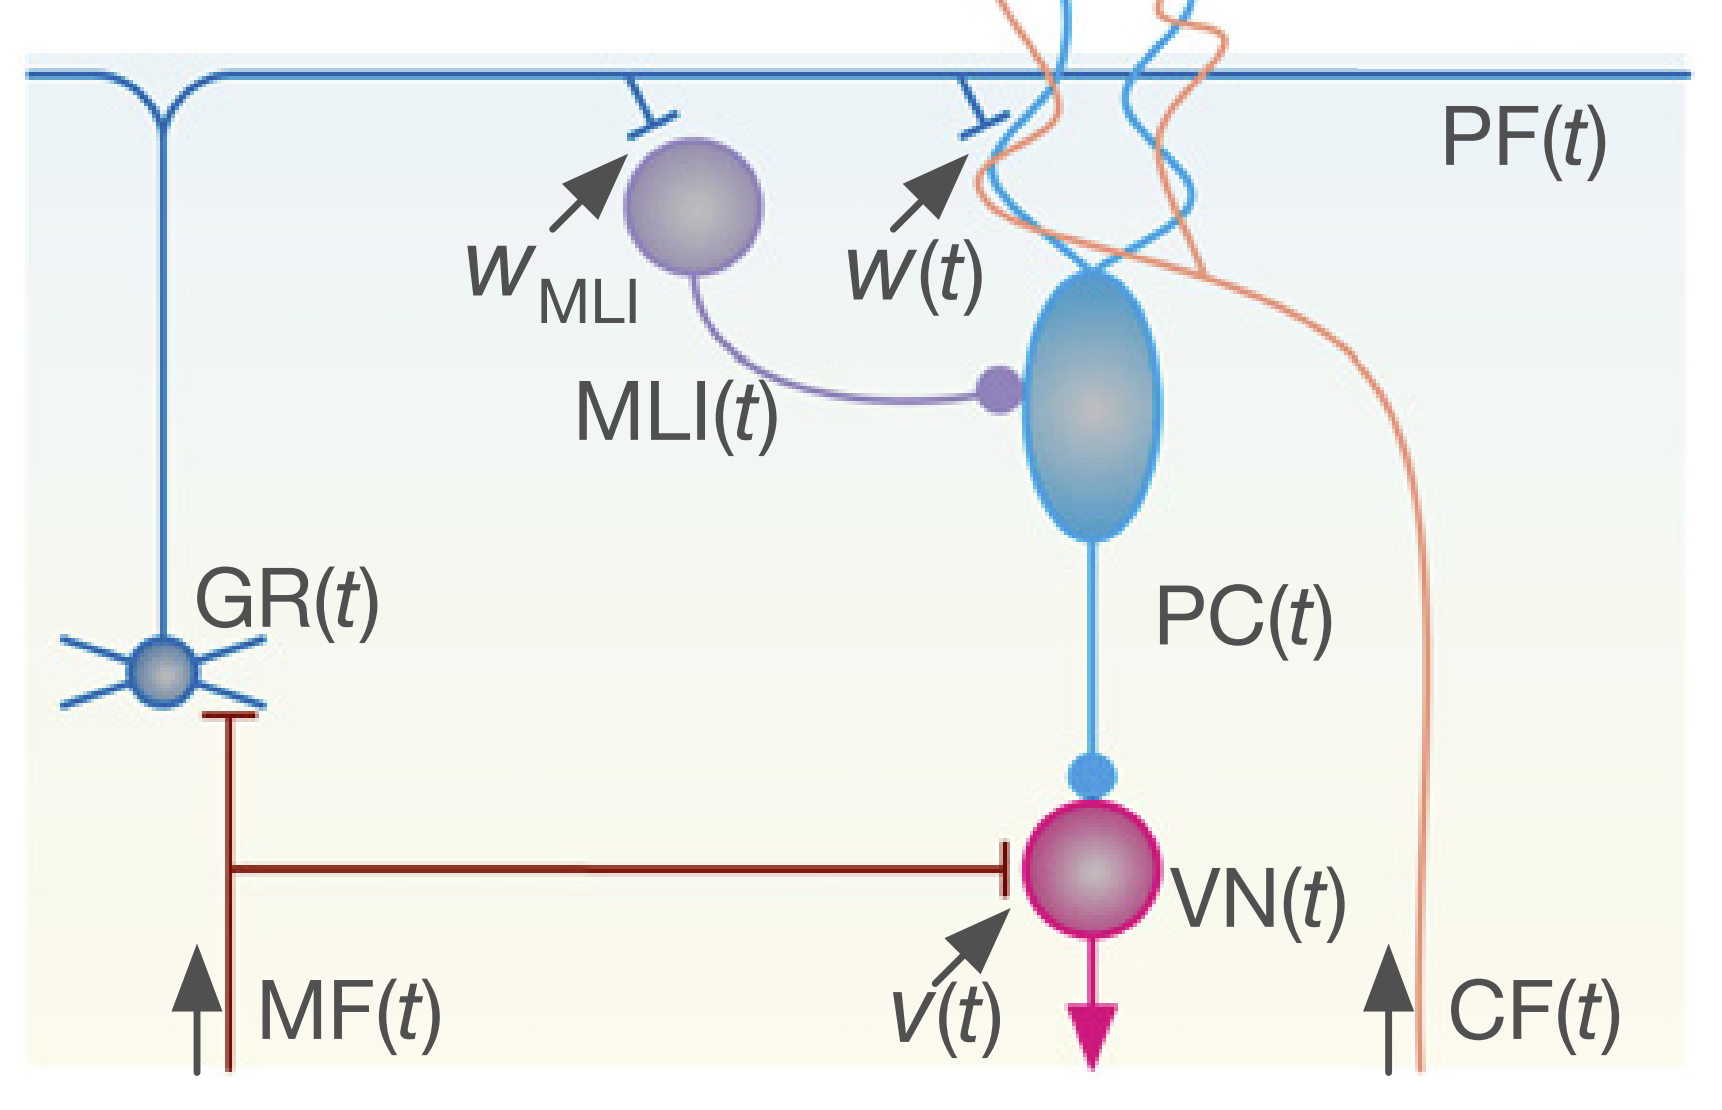
\includegraphics[scale=0.7]{images/cerebellar_network.png}
    \caption{Diagram of a simplified neuronal network modelling the cerebellar network underlying OKR gain, from Figure 1A of \cite{yamazaki2015modeling}.}
    \label{fig:CerebellarNet}
\end{figure}



\subsection{Motor Learning of OKR}

There are two primary mechanisms behind the plasticity of synaptic weight in the brain: long-term potentiation (LTP) and long-term depression (LTD). Long-term potentiation is a process of strengthening synaptic weights, and long-term depression is a process of weakening synaptic weights.

There are competing hypotheses regarding the neural underpinnings of motor learning in the neural cortex.  While the complete mechanisms are unknown, the longstanding Marr-Albus-Ibo hypothesis suggests that motor learning is caused by LTD at the PF-PC synapses. However, there is a competing hypothesis from Miles and Lisberger, who suggest that LTP at the MF-VN synapses is the underlying mechanism of motor training of the vestibuloocular reflex. However, these hypotheses need not be considered in isolation. The inspiration behind the work of Yamazaki et. al. is evidence from studies of OKR training which suggest that both PF-LTD and MF-LTP are important to motor learning \cite{yamazaki2015modeling}.This is the central hypothesis we are seeking to support with this project. MF-LTP and PF-LTD need not be considered in competing hypotheses regarding the mechanisms central to motor learning. They are compatible and complementary mechanisms.

\section{Methods}

\subsection{Modeling the Cerebellar Network}

We will first use the neuronal network structure of Figure \ref{fig:CerebellarNet} to derive equations modelling OKR gain based on the plasticity of PF-PC and MF-VN synapses. These derivations follow those from the \cite{yamazaki2015modeling}, so here I strive for a balance of detail where the origins are clear but do not take up too much time. The full derivations can be found in the original text and it's supporting information.

\subsubsection{Cellular Activation}

We begin by deriving functions for the activation of the various cells in the network. Here, we are considering population activation of cell types.

We will start by determining the activation of the Purkinje cells. PCs receive excitatory input from the granule cells via the parallel fibers, weighted by synaptic weight $w(t)$, and  inhibitory input from molecular-layer interneurons, yielding 
\begin{equation}
    \label{1}
    PC(t) = w(t)GR(t)-MLI(t)+PC_0,
\end{equation}
where $PC_0$ represents spontaneous activation of the PCs.

MLIs also receive input from granule cells via parallel fibers, with synaptic weight $w_{MLI}$, \begin{equation}
    \label{2}
    MLI(t) = w_{MLI}GR(t).
\end{equation}

For simplicity, the authors assume the granule cells simply relay signals from the mossy fibers, \begin{equation}
    \label{3}
    GR(t) = MF(t).
\end{equation}

Substituting \eqref{2} and \eqref{3} into \eqref{1} and simplifying, we now have the population activity of Purkinje cells as \begin{equation}
    \label{4}
    PC(t) = MF(t)(w(t)-w_{MLI}) + PC_0
\end{equation}

We derive the activation of vestibular nuclear neurons in a similar manner. VNs recevive excitatory input from mossy fibers, with synaptic weight $v(t)$, and inhibitory input from Purkinje cells, yielding 
\begin{equation}
    \label{5}
    VN(t) = v(t)MF(t) - PC(t) + VN_0,
\end{equation}

where $VN_0$ is spontaneous activation of VNs. Substituting \eqref{4} into \eqref{5} and simplifying yields \begin{equation}
    \label{6}
    VN(t) = MF(t)(v(t)-w(t)+w_{MLI}) - PC_0 + VN_0.
\end{equation}

We next expand the activation of mossy fibers into \(MF(t) = \overline{MF} + \delta MF(t)\), where \(\overline{MF}\) is the mean activity and \(\delta MF(t)\) is the fluctuation around the mean. This allows us to rewrite \eqref{6} as \begin{equation}
    \label{7}
    VN(t) = \overline{MF}(v(t)-w(t)+w_{MLI}) + \delta MF(t)(v(t)-w(t)+w_{MLI}) - PC_0 + VN_0.
\end{equation}

\subsubsection{OKR gain}

We are now able to derive the equation for OKR gain. The movement of the eye is proportional to the \textit{modulatory} activity of the VNs, so we consider the nonconstant part of \eqref{7} to get \begin{equation}
    \label{8}
    EYE(t) = g_{EYE}\delta MF(t)(v(t)-w(t)+w_{MLI}),
\end{equation}
where $g_{EYE}$ is a constant which translates from neural activtiy to eye movement.

Finally, we define OKR as the maximum amplitude of this eye movement, \begin{equation}
    \label{9}
    OKR(t) = g_{OKR}(v(t)-w(t)+w_{MLI}),
\end{equation}
where \(g_{OKR} = 2\cdot \max(\delta MF(t))\).

\subsubsection{Synaptic Weights}

We now must derive the differential equations for the synaptic weights, $v$ and $w$, which drive the model.

We begin with the PF-PC synapses. These synapses experience spontaneous decay, LTP triggered by GRs (via PFs), and LTD triggered by the combined activity of GRs and CFs. This yields the differential equation \begin{equation}
    \label{10}
    \tau_w \frac{dw}{dt} = -w(t) + \braket{GR(t)} - \braket{GR(t)CF(t)},
\end{equation} 
where the notation \(\braket{f(t)}\) denotes the temporal average of \(f\).

Similarly to how we derived the activity of PCs and VNs, we can substitue \eqref{3} and expand \(MF(t) = \overline{MF} + \delta MF(t)\) and \(CF(t) = \overline{CF} + \delta CF(t)\). Temporal averages are assumed to be over a short enough time span so that the fluctuation of activity, in this case \(\braket{\delta MF(t)}\), is 0. Knowing this, we can take advantage of the linear nature of expectation to derive
\begin{equation}
    \label{11}
    \tau_w \frac{dw}{dt} = -w(t) + (\overline{MF}-\overline{MF}\ \overline{CF}) - \braket{\delta MF(t) \delta CF(t)}.
\end{equation}

We now have two cases to consider. During training, the fluctuation in MF and CF activity are correlated so we cannot reduce the final term. However, at rest, $\delta MF(t)$ and $\delta CF(t)$ are independent, so this final term reduces to 0. Finally, changes during training are must faster than during recovery, so we consider two separate time constants for each case. We now have the update equation for the PF-PC synaptic weight, 
\begin{equation}
    \label{12}
    \frac{dw}{dt} = \begin{cases}
    \frac{1}{\tau_{learn}}(-w(t)+w_0-c_{OKR}) & \text{(during training)} \\
    \frac{1}{\tau_{recov}}(-w(t)+w_0) & \text{(after training)}
    \end{cases}
\end{equation}
where \(\tau_{learn}\ll \tau_{recov}\), \(c_{OKR} \equiv  \braket{\delta MF(t) \delta CF(t)}\), and \(w_0\equiv \overline{MF}-\overline{MF}\ \overline{CF}\) is the baseline synaptic weight at rest.

Finally, we derive the update equation for the MF-VN synapse. We start by considering the equation
\begin{equation}
    \label{13}
    \tau_v \frac{dv}{dt} = -\braket{MF(t)v(t)} + \braket{MF(t)(VN(t)-\theta(t))},
\end{equation}
where the first term represents LTD of the synapse triggered by activation of the mossy fibers, and the second term represents Hebbian learning at the MF-VN synapse. \(\theta(t)\equiv\braket{VN(t)}\) is a parameter representing the postsynaptic activity, which determines whether LTP or LTD is occurring at the synapse.

Substituting this definition of \(\theta(t)\) and further substituting for \(VN(t)\) with \eqref{7}, we can derive \begin{equation}
    \label{14}
    \tau_v \frac{dv}{dt} = -\overline{MF} v(t) + \braket{\delta MF(t) \delta MF(t)}(v(t)-w(t)+w_{MLI}).
\end{equation}

Assuming spiking of the MF follows a Poisson distribution, we can use the fact that Poisson distributions have equal mean and variance to simplify \(\braket{\delta MF(t) \delta MF(t)} = \overline{MF}\). This substitution, plus the final assumption that \(\overline{MF}=1\) for simplicity, yields the final differential equation for the MF-VN synaptic weight,
\begin{equation}
    \label{15}
    \frac{dv}{dt} = \frac{1}{\tau_v}(-w(t)+w_{MLI}).
\end{equation}

Thus, \eqref{9}, \eqref{12}, and \eqref{15} give us the defining equations for the system under normal conditions.

The values of constants are provided in the original paper, were they were fit to experimental data of OKR gain training. These values are \(v(0)=1\), \(w(0)=w_0=1\), \(c_{OKR}=0.3\), \(\tau_{learn}=20\) minutes, \(\tau_{recov}=2.5\) hours, \(\tau_{v}=5.5\) hours, and \(g_{OKR}=0.3\).

\subsection{Massed vs Spaced Training}

The first experiment simulated in the paper is the effect of massed vs. spaced training. This is to recreate real-world experimental evidence in which the final OKR gain after post-training recovery was greater after a series of shorter, spaced training sessions as opposed to one long train session. In particular, we simulate OKR gain adaptation using \eqref{9}, \eqref{12}, and \eqref{15} under 4 training regimes with equal total training time: 1 hour of massed training, 4 training sessions of 15 minutes each spread over a 4 hour period, 4 training sessions of 15 minutes each spread over a 4 day period, and 8 training sessions of 7.5 minutes each spread over an 8 day period.

\subsection{Genetically Modified Mice}

The other experiment of the original paper we seek to recreate is the effect of genetic modifications of mice on OKR training. The governing equations of these models are slightly different from the original case, so we derive them below. 

\subsubsection{PF-LTP-Deficiency}

Without a functioning PF-LTP mechanism, the synaptic weights of the PF-PC synapses can only decrease, resulting in a steady-state synaptic weight of 0. We assume for all these equations that the steady-state has already been reached. Thus, \begin{equation}
    \label{16}
    w(t)=w(0)=0.
\end{equation}

Additionally, in the absense of inhibition from Purkinje cells, the vestibular nuclear neurons experience synaptic strengthening at the MF-VN synapse via Hebbian learning. We again assume that this has already reached steady-state at the start of simulation, so \begin{equation}
    \label{17}
    v(t)=v(0)>0.
\end{equation}

Finally, with the absence of synaptic input from PCs, the activity of VNs, and thus the calculated OKR gain, depends only on the synaptic weight of the MF-VN synapses, \begin{equation}
    \label{18}
    OKR(t)=g_{OKR}v(t)=g_{OKR}v(0).
\end{equation}

Thus, in the case of deficiency in PF-LTP, OKR gain cannot be trained, and instead remains constant.

\subsubsection{Spontaneous PF-LTD-Deficiency}

We next consider the case of genetic deficiencies in spontaneous PF-LTD. Spontaneous PF-LTD is represented by the \(-\overline{MF}\ \overline{CF}\) term in \(w_0\). When the mechanism is deficient, the baseline weight of the PF-PC synapses is thus simply \(w_0 = \overline{MF}\). The PF-PC synapses follow the same update rule as in the normal case, \eqref{12}, just with the different constant.

With this stronger weight, the Purkinje cells are more active, and inhibit the vestibular nuclear neurons so that \(VN(t)=0\) at resting conditions. The vestibular nuclear neurons can only become active, and thus the optokinectic response can only occur, if \(v(t)-w(t)+w_{MLI} \ge 0\), adding a condition to \eqref{9}, \begin{equation}
    \label{19}
    OKR(t) = \begin{cases}
        g_{OKR}(v(t)-w(t)+w_{MLI}) & \text{if }v(t)-w(t)+w_{MLI} \ge 0\ \\
        0 & \text{otherwise.}
    \end{cases}
\end{equation}

Additionally, Hebbian learning at the MF-VN synapse only occurs if the VNs are active, so the same condition is added to the update rule for \(v\), \begin{equation}
    \label{20}
    v(t) = \begin{cases}
        \frac{1}{\tau_v}(-w(t)+w_{MLI})& \text{if }v(t)-w(t)+w_{MLI} \ge 0\ \\
        0 & \text{otherwise.}
    \end{cases}
\end{equation}

The update rule for \(w\) remains the same, although recall that the baseline weight being higher modifies the dynamics of the system. Since \(w_0\) represents the balanced state between spontaneous PF-LTP and PF-LTD, the authors use the higher value \(w(0)=w_0=1.1\) for this case. Additionally, they assume that there exist some compensation mechanism to allow motor training to still occur in PF-LTD deficient animals, which is represented by changing the parameter \(c_{OKR}\) to 1.

\subsubsection{Depletion of GABA Receptors in Purkinje Cells}

The final case considered in the original text is the depletion of GABA receptors in Purkinje cells. GABA receptors are where PCs receive inhibitory input from MLIs, so when these receptors are depleted, this synaptic weight disappears from consideration. This is modelled by setting the constant weight \(w_{MLI}=0\). This leads to greater activity in the PCs, and thereby greater inhibition of the VNs. To keep OKR gain positive, the authors added a compensating constant, \(c_{compensate}=1\), yielding the equation
\begin{equation}
    \label{21}
    OKR(t) = g_{OKR}(v(t)-w(t))+c_{compensate}.
\end{equation}

The PF-PC and MF-VN synaptic weights follow their normal update rules, \eqref{12} and \eqref{15}, although it is noteworthy that since Extending the \(w_{MLI}=0\), the update rule for \(v\) simplifies to \begin{equation}
    \label{22}
    \frac{dv}{dt} = \frac{1}{\tau_v}(-w(t)).
\end{equation}

\subsection{Extending the Model}

We now explain the ways in which we expanded on the model presented by the paper for deeper understanding.

\subsubsection{The Effect of Time Constants}

We first simulated the effects of the time constants on OKR gain adaptation. Although this is not necessarily based on existing physiological evidence such as the experiences . If it is possible to have genetic modifications which lead to total deficiencies in PF-LTP and PF-LTD, it is feasible that there are also genetic modifications which could strength or weaken the process without shutting it down completely.

These simulations were done for all three time constants, \(\tau_v\), \(\tau_{learn}\), and \(\tau_{recov}\). When testing each time constant, the normal values described in section 2.1.3 were used for the other two time constants. \(\tau_{learn}\) was varied from 1 minute to 40 minutes, \(\tau_{recov}\) was varied from 1 hour to 2.5 hours, and \(\tau_v\) was varied from 1 hour to 10 hours. After simulations, the final OKR gain values were plotted against the varied time constants.

\subsubsection{Massed vs. Spaced Training with LTD-Deficiency}

We next combined aspects of the original experiments, by simulating the effects of various training protocols in the case of PF-LTD deficient mice. This was done in a similar as the experiment of section 2.2, however with slightly different training regimes. Again, each regime consisted of 1 hour of total training. These regimes were: 1 hour of mass training, 20 minute training sessions every 8 hours, 15 minute training sessions every 6 hours, and 10 minute training sessions every 4 hours. Training sessions were aligned so that the final training session ended at the same time. We also use the modelling equations \eqref{19} and \eqref{20} from section 2.3.2 to run the simulations. The final values of OKR gain after 1 hour of recovery following the final training session, rather than after total recovery as in the case of normal conditions, since OKR gain would return to 0 in all cases with total recovery.

We expect to see that the spaced training paradigms will yield larger increases in OKR gain, as in normal mice. However, since we expect that long-term memories are not consolidated in the case of LTD-deficiency, these benefits will be short-lasting.

\subsubsection{Combining Genetic Deficiencies}

Finally, we simulated training of mice which are both deficient in PF-LTD and have depletion of the GABA receptors in the Purkinje cells. This was done by considering equations \eqref{19} and \eqref{20}, and setting \(w_{MLI}=0\) as was the case in section 2.3.3. We again add a term \(c_{compensate}\) to make up for the negative OKR values. This yields the equations \begin{equation}
    \label{23}
    OKR(t) = \begin{cases}
        g_{OKR}(v(t)-w(t)) + c_{compensate} & \text{if }v(t)-w(t) \ge 0\ \\
        0 & \text{otherwise}
    \end{cases}
\end{equation} and \begin{equation}
    \label{24}
    v(t) = \begin{cases}
        \frac{1}{\tau_v}(-w(t))& \text{if }v(t)-w(t) \ge 0\ \\
        0 & \text{otherwise.}
    \end{cases}
\end{equation}

Seeing as we expect each of these deficiencies individually to result in short-term memory formation, but no long-term memory consolidation, we expect to see similar effects here. We expect very small increases in OKR gain to occur during training, but for OKR gain to return to the same baseline level after recovery.

\subsection{Implementation}

Models were simulated in MATLAB using Forward Euler's method with a time step of 1 minute. Training regimes were simulated with boolean functions which indicate whether training is occurring at a given time, allowing for the casewise behavior of \(\frac{dw}{dt}\). The recreated models largely followed the logical structure of the C implementation from the original paper \cite{yamazaki2015modeling}.

\section{Results}

\subsection{OKR adaptation under normal conditions}

We will first analyze the simulation results of OKR adaptation under normal conditions. The simulated OKR gain and synaptic weights over a nine day period containing five days of one hour trainings are shown in the plots below. Our results are consistent with those of the original paper.

\begin{figure}[h]
    \centering
    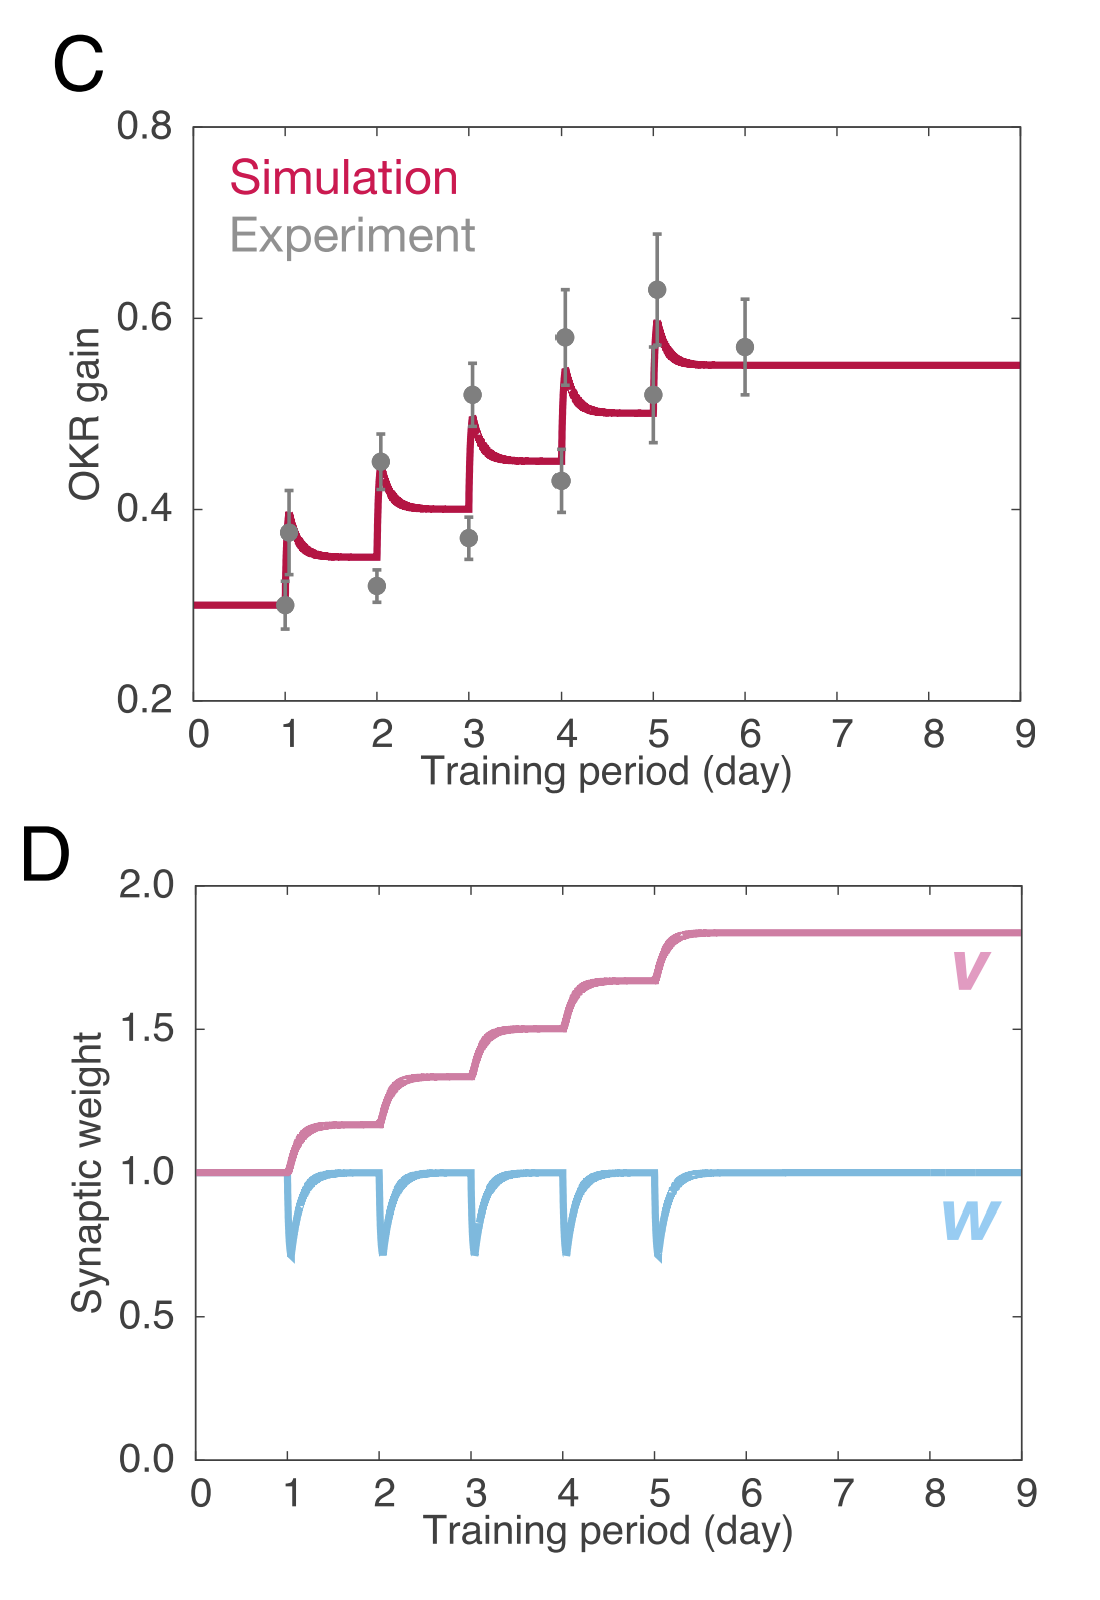
\includegraphics[scale=0.58]{images/normal_operations_orig.png}
    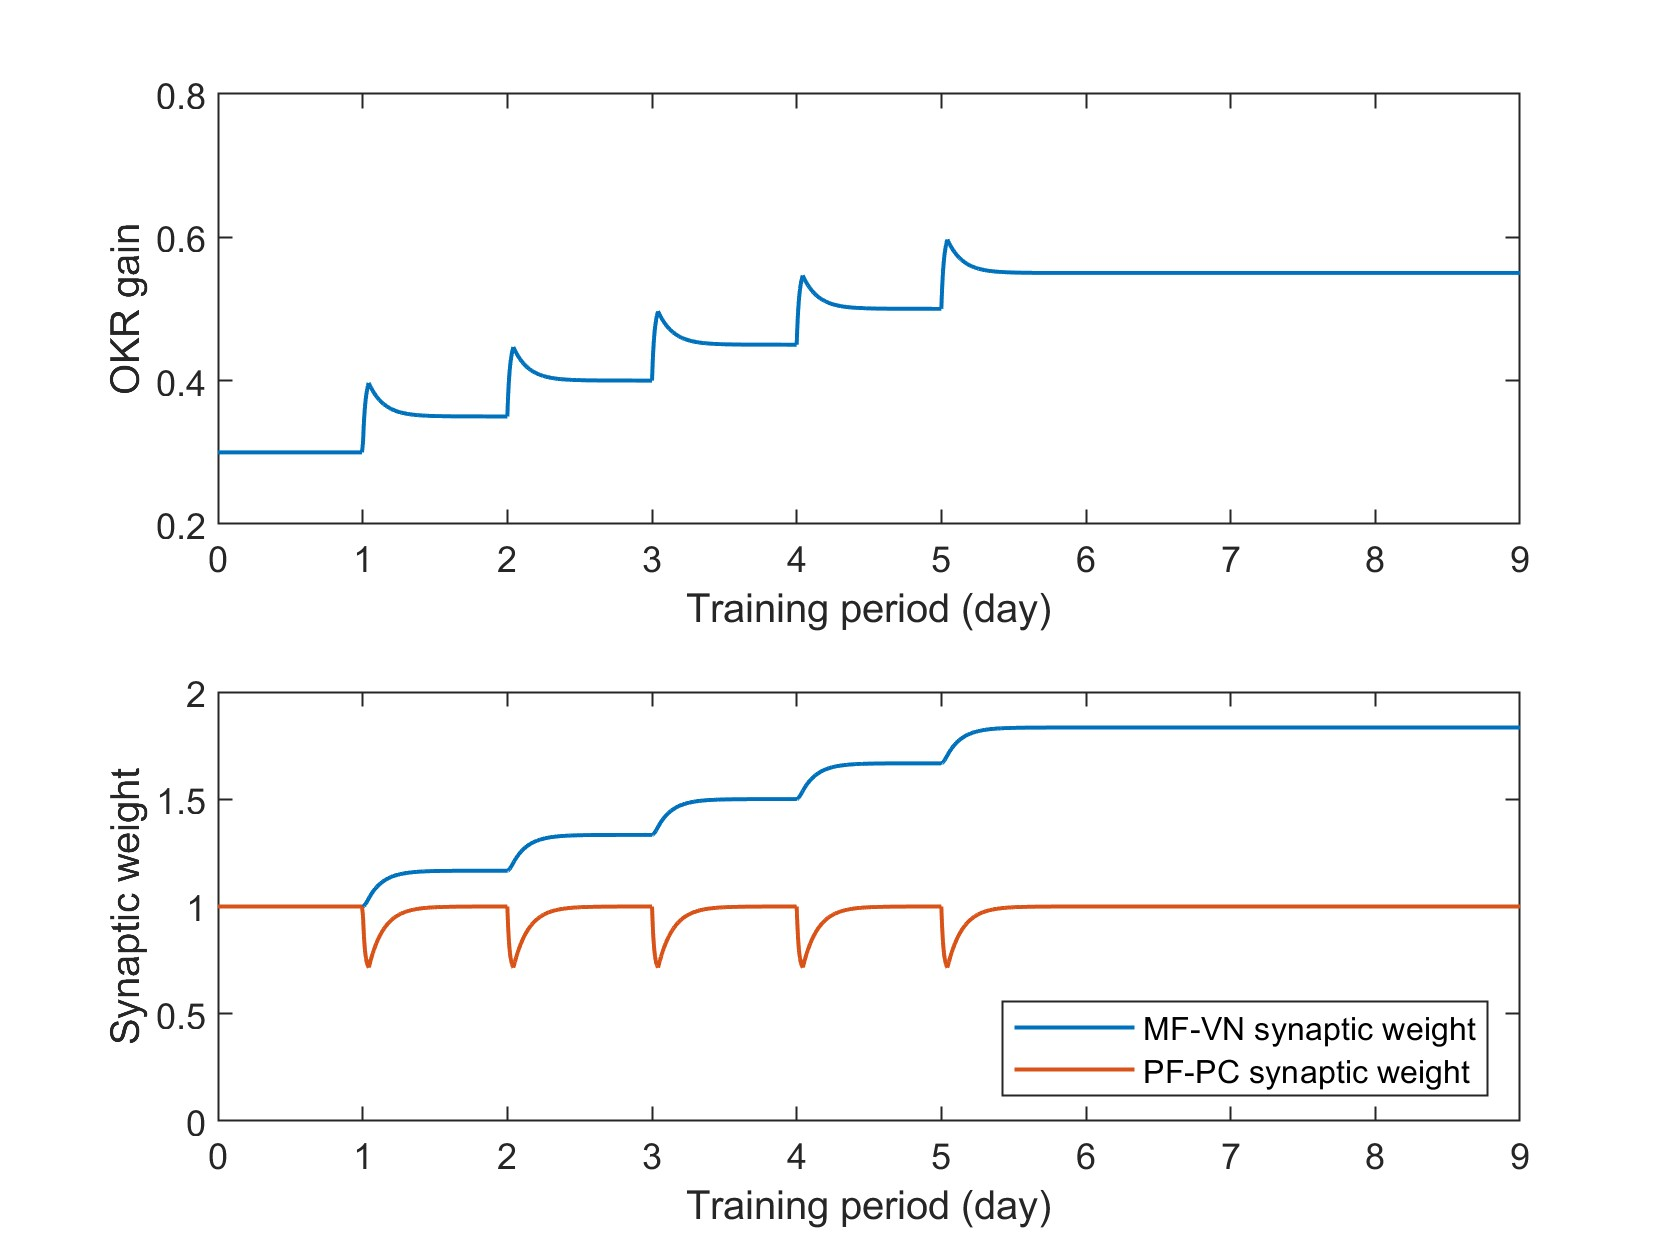
\includegraphics[scale=0.18]{images/Fig1_rec.jpg}
    \caption{OKR gain and synaptic weights over nine days, with training occurring for one hour a day for five days. On the left are Figures 1C and 1D from \cite{yamazaki2015modeling}, and on the right are the recreated plots from our MATLAB simulation.}
    \label{fig:normal_okr_adaptation}
\end{figure}

We can see that during the training periods, there are sharp increases in OKR gain. On the neural level, these changes coincide with sharp decreases in the synaptic weight of the PF-PC synapses, and increases in the synaptic weight of the MF-VN synapses. Following training, the PF-PC synaptic weight gradually returns to its baseline weight. The MF-VN synaptic weight continues to gradually increase, eventually levelling of as the PF-PC synaptic weight has returned to baseline. Finally, OKR gain gradually decreases during the recovery period, eventually settling at a steady value higher than that before training, but lower than the peak during training.

\subsection{Massed vs Spaced Training}

We next observe the results of simulating normal OKR gain adaptation under various training regimes.

\begin{figure}[h]
    \centering
    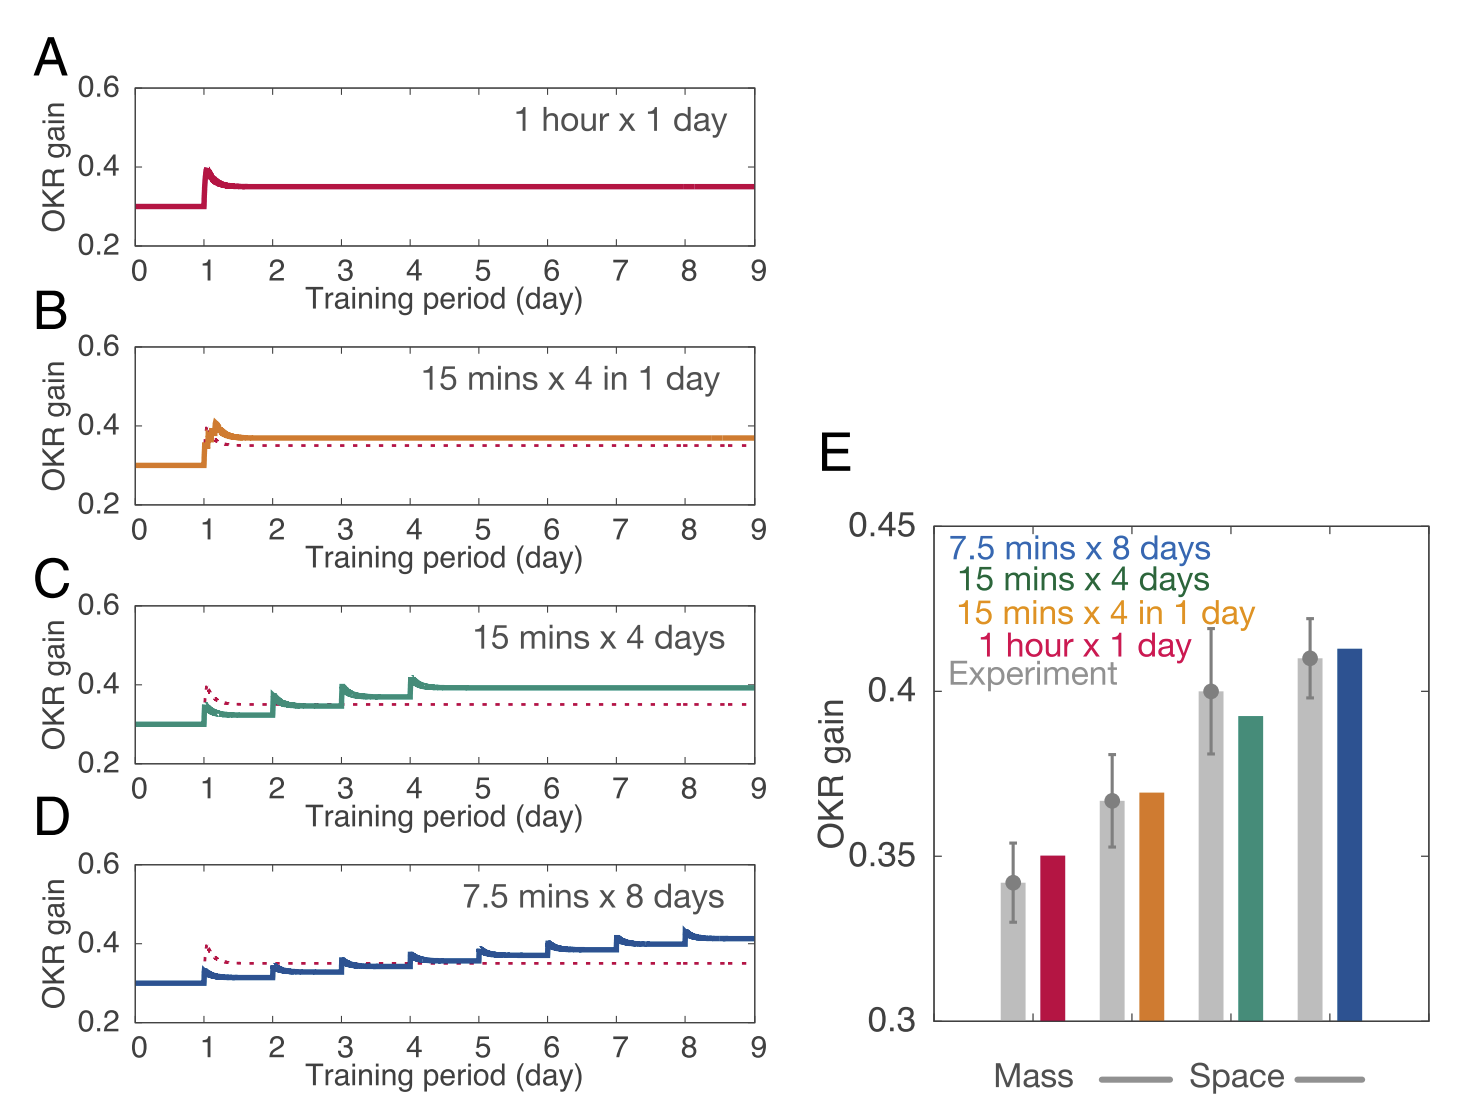
\includegraphics[scale=0.60]{images/Fig3_orig.png}
    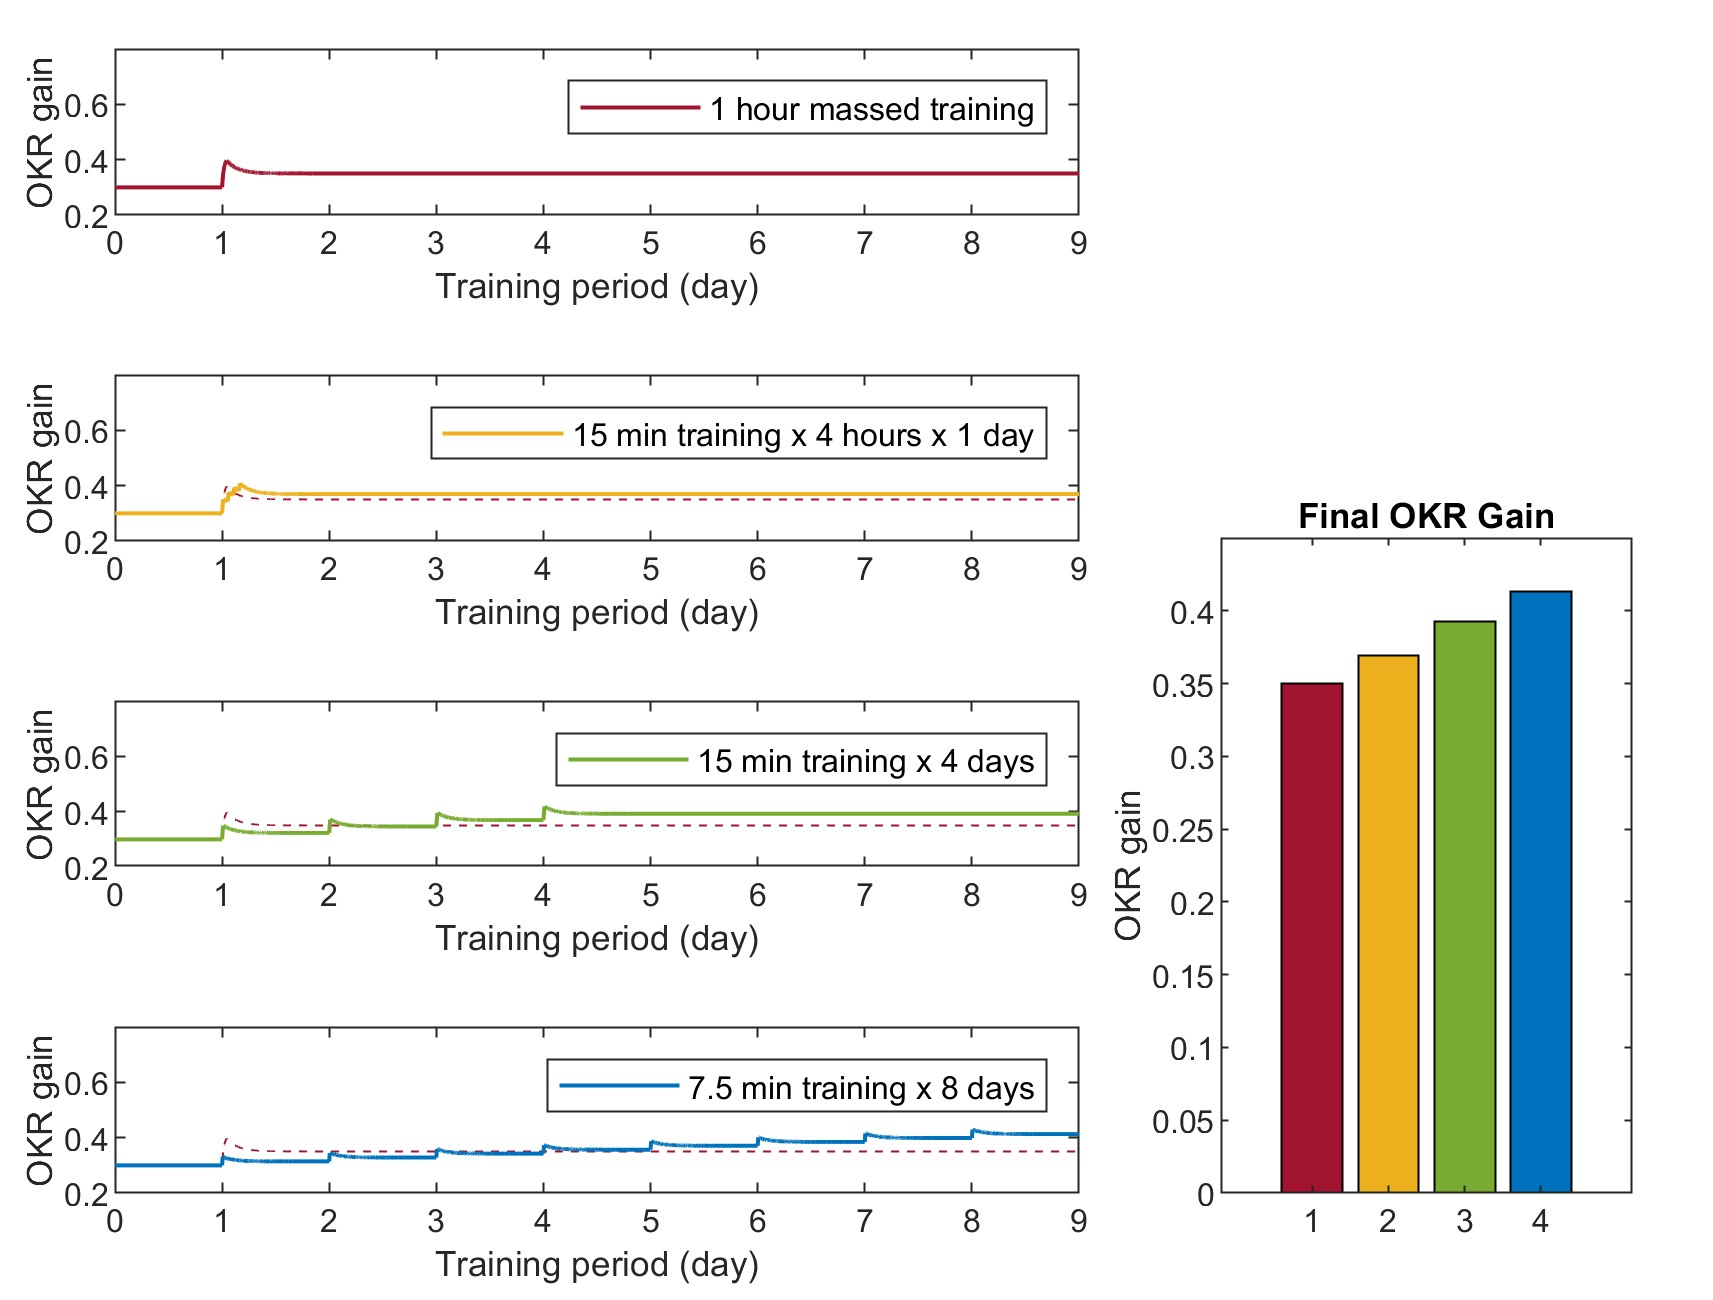
\includegraphics[scale=0.12]{images/Fig3_rec.jpg}
    \caption{OKR gain adaptation following a massed training paradigm vs various spaced training paradigms. The line plots depict OKR gain levels over a nine day period for each training regime. The bar plot compares the final OKR gain value for each training regime. The left plots are from Figure 3 of \cite{yamazaki2015modeling}, and the right plots are our recreations from our MATLAB simulation.}
    \label{fig:mass_vs_spaced_training}
\end{figure}

We observe the same patterns in OKR gain during and after training as we did in Figure \ref{fig:normal_okr_adaptation}. However, observing the bar graph comparing the final OKR gain values after recovering from all training, it is evident that the shorter, spaced training sessions yielded more effective results in training the optokinetic response. These results are again consistent with those of the original paper.

Here, taking the entire hour of training in one single session yielded the smallest over gain in OKR gain. Splitting the training into 4 sessions of 15 minutes, each starting on consecutive hours, yielded the next best results. Spacing these training sessions further apart, with sessions spaced by a day rather than an hour, yielded even larger gains. Finally, splitting into even shorter sessions spaced by the day to allow for full recovery time yielded the best results of all simulations.

\subsection{Genetically Modified Mice}

Here we show our final recreated figure of the original paper, demonstrating the results of training genetically modified mice. Note that these plots depict change in OKR gain rather than proper values. This is because, unlike other models in the original paper, this one is not fit to experimental data \cite{yamazaki2015modeling}.

\begin{figure}[h]
    \centering
    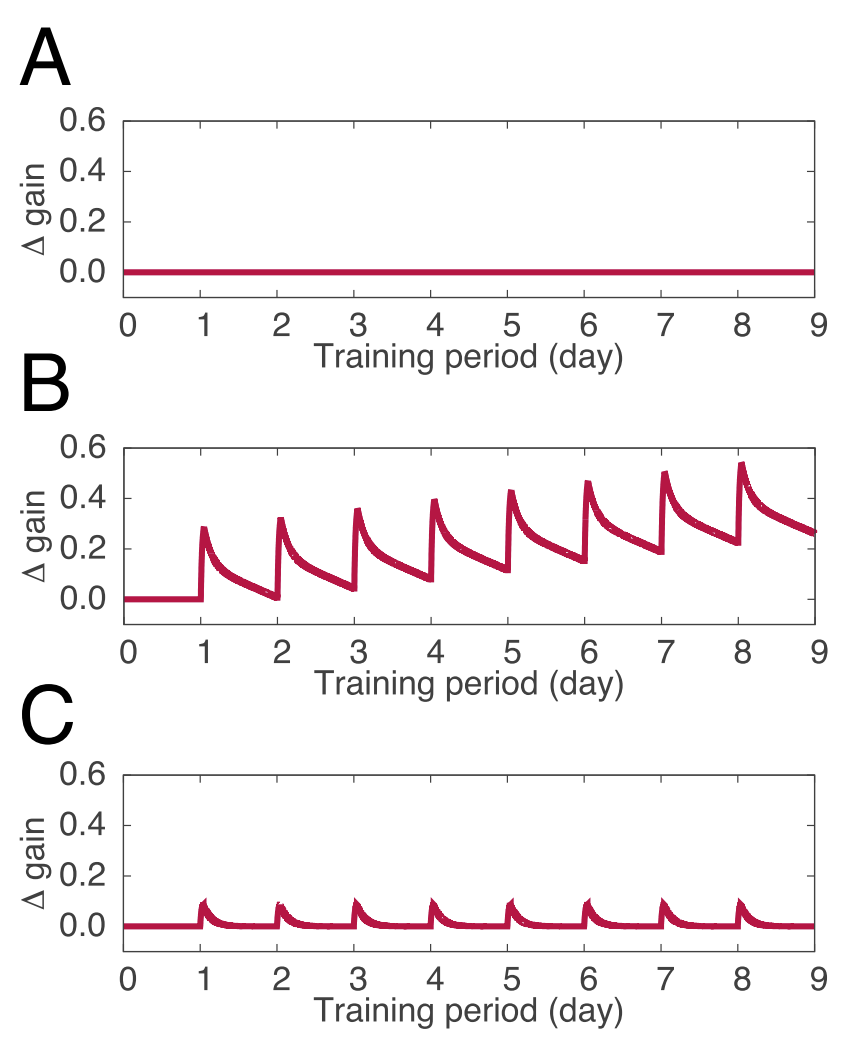
\includegraphics[scale=0.7]{images/Fig4_orig.png}
    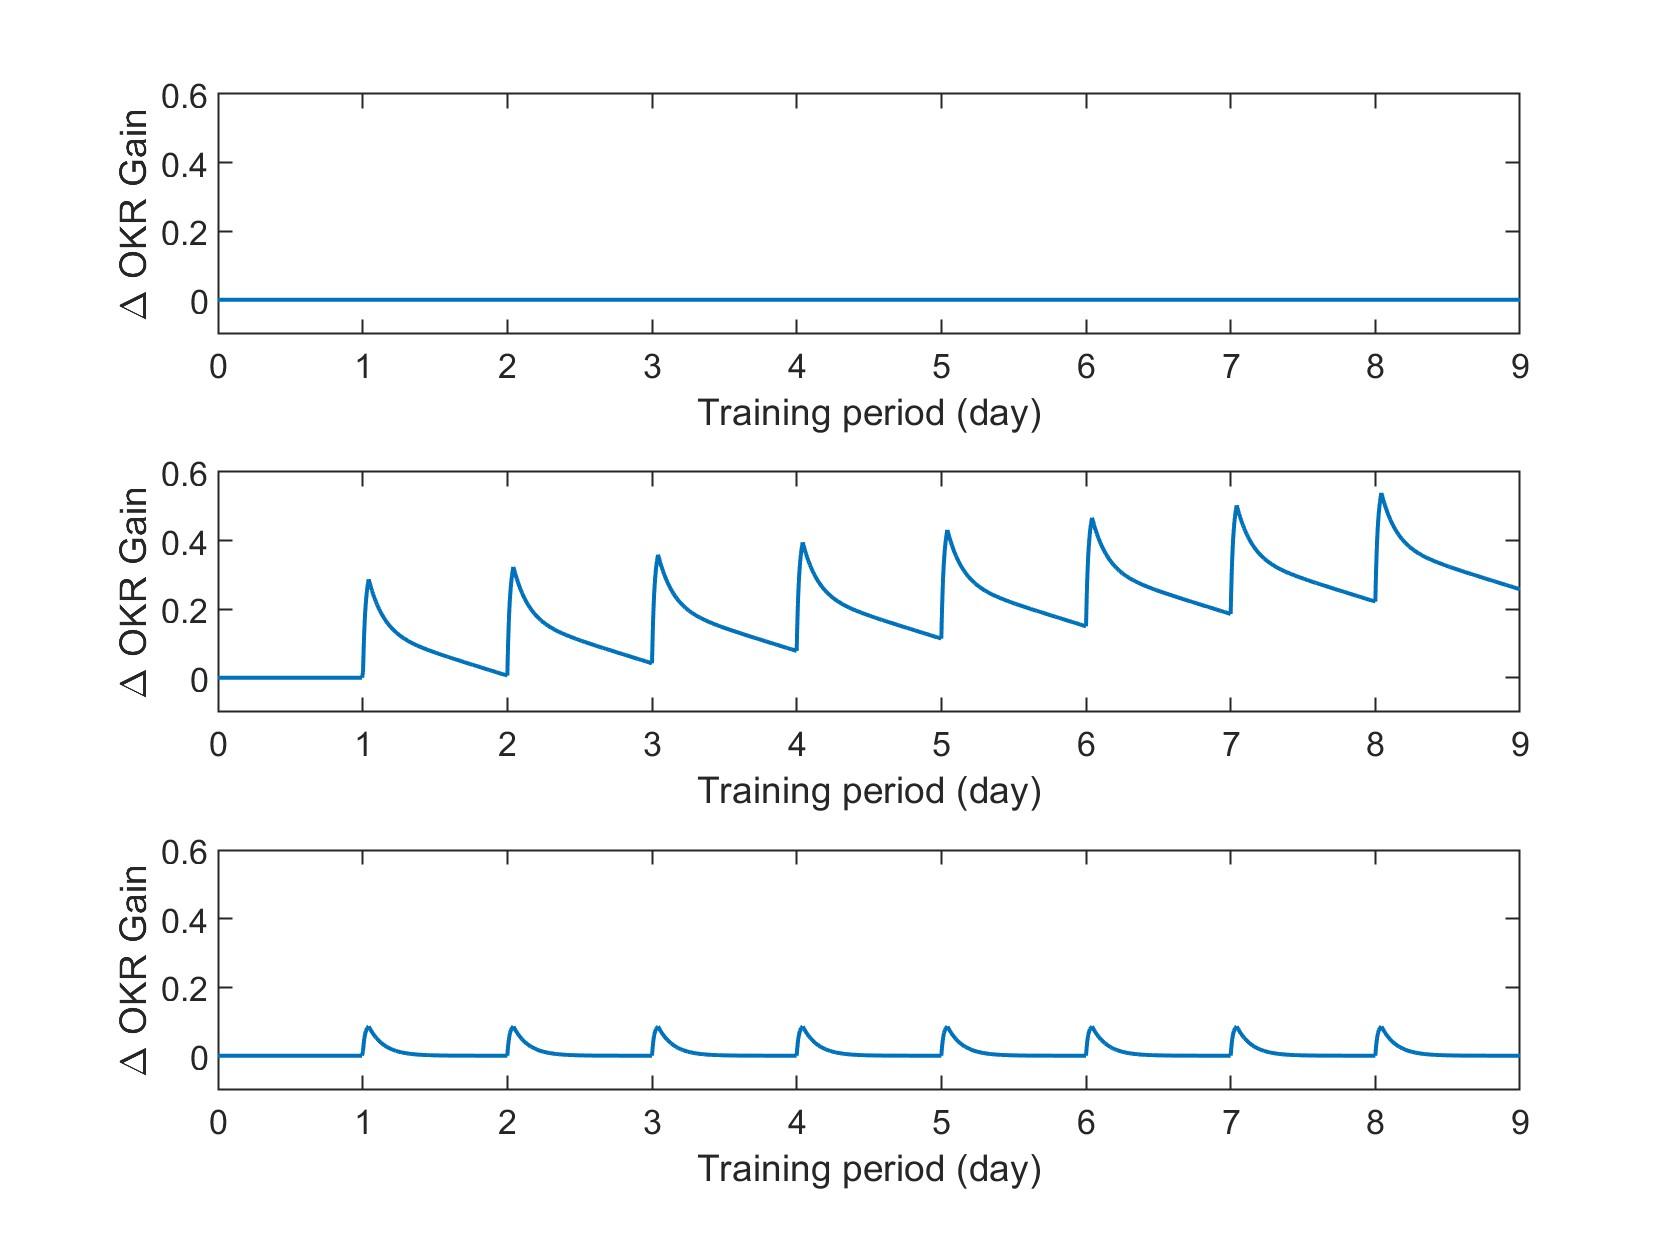
\includegraphics[scale=0.14]{images/Fig4_rec.jpg}
    \caption{The effects of various genetic manipulations on OKR training. The top plots depict training a mouse with deficiencies in PF-LTP. The middle plots depict training a mouse with deficiences in spontaneous PF-LTD. The bottom plots depict training a mouse with depleted GABA receptors in Purkinje cells. The left plots are from Figure 4 of \cite{yamazaki2015modeling}, and the right plots are from our recreated MATLAB simulation.}
    \label{fig:gene-modified_training}
\end{figure}

The topmost plots depict attempts at training mice with genetic deficiencies in PF-LTP. Here, OKR gain remains constant regardless of training, as expected by the derivation of \eqref{18}.

The middle plots depict training of mice with deficiencies in spontaneous PF-LTD. Here, OKR gain sharply spikes during training, as in the normal case. However, during recovery, OKR gain continiously decreases, rather than reaching a steady value as it did in Figure \ref{fig:normal_okr_adaptation}.

The bottom plots depict training of mice with depleted GABA receptors in Purkinje cells. In this case, only moderate increases in OKR gain occur during training, and these gains are lost during the recovery periods.

\subsection{Extensions}

\subsubsection{The Effect of Time Constants}

Here are the plots of OKR gain vs each time constant.

\begin{figure}[h]
    \centering
    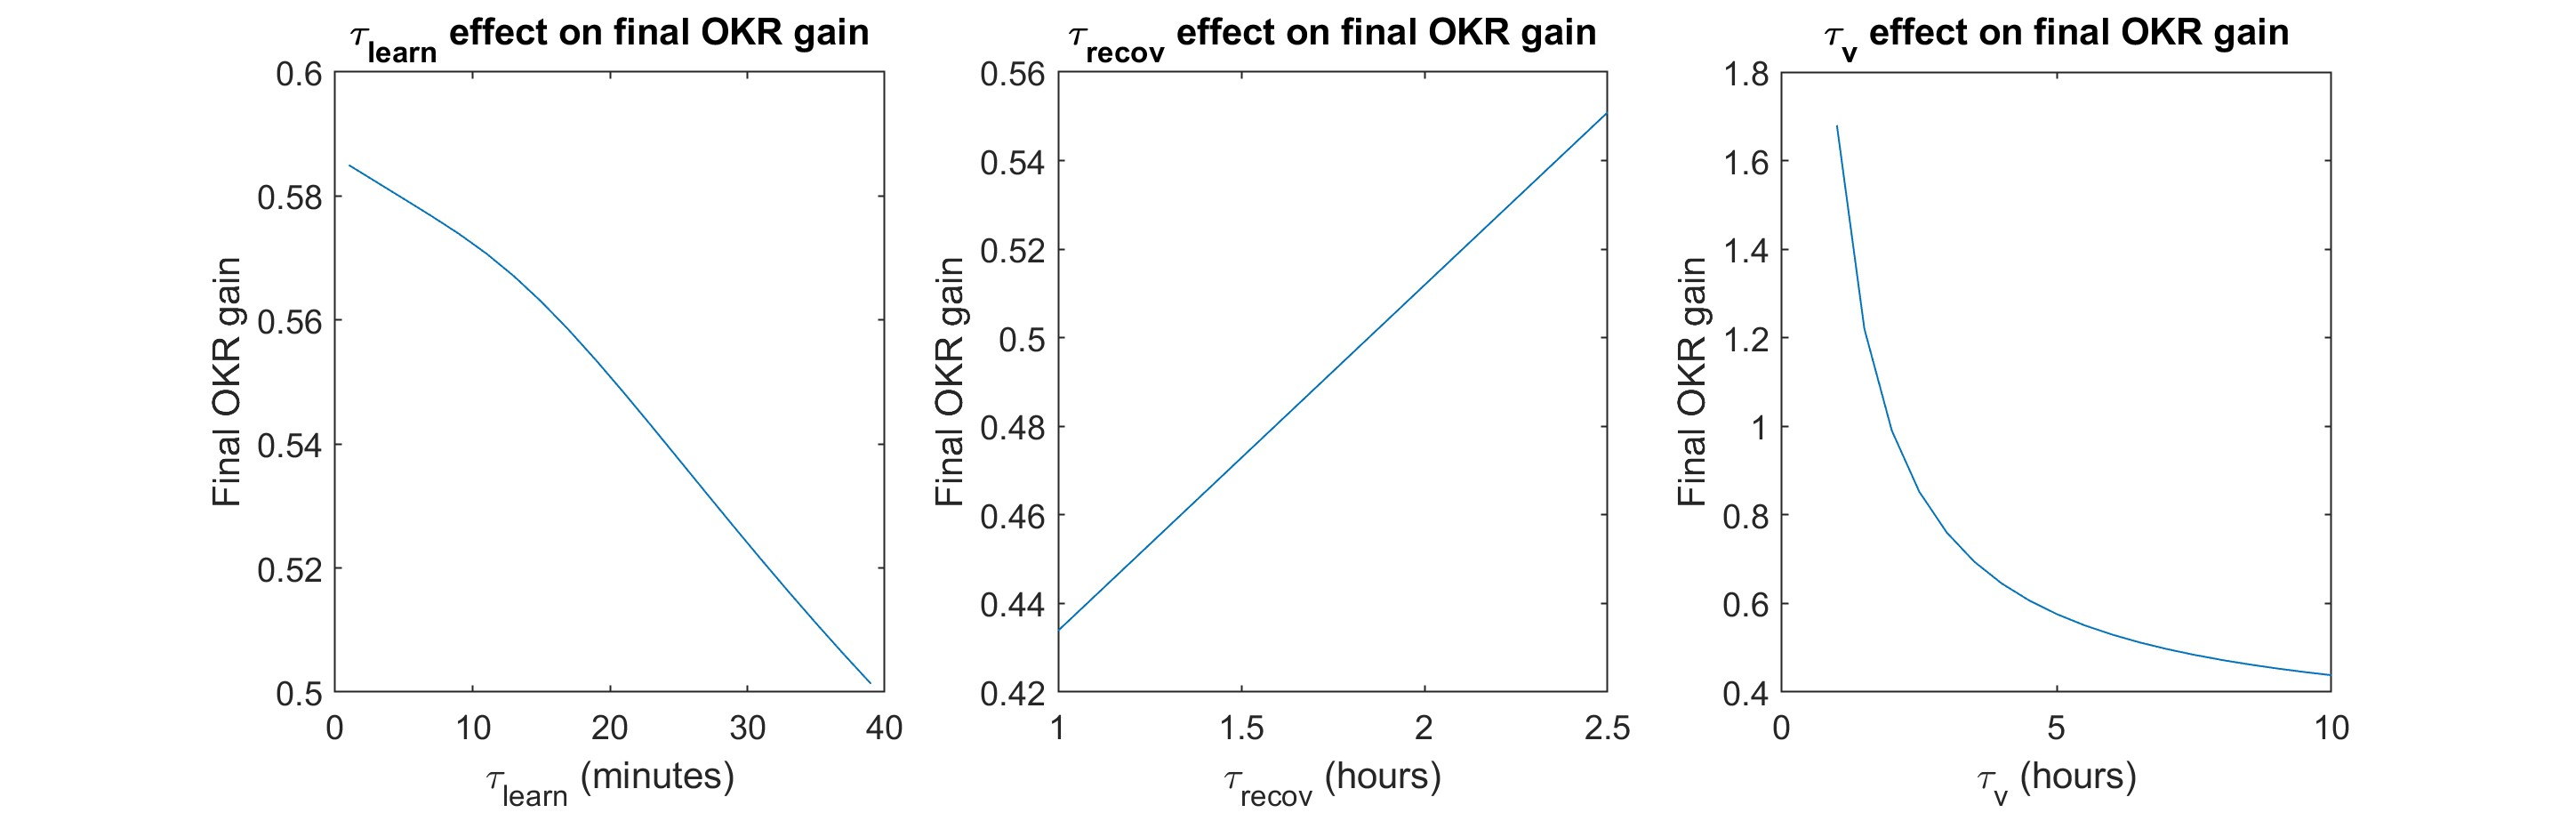
\includegraphics[scale=0.15]{images/effect_of_time_constants.jpg}
    \caption{The relationships between each of the time constants and training of the optokinetic response.}
    \label{fig:time_constants}
\end{figure}

The first and third plots indicate the \(\tau_{learn}\) and \(\tau_v\) each have an inverse relationship with OKR gain. The middle plot shows a positive linear relationship between \(\tau_{recov}\) and OKR gain.

\subsubsection{Massed vs. Spaced Training with LTD-Deficiency}

The next page contains the plots comparing OKR gain adaptation under various training regimes for simulated mice with genetic deficiencies in PF-LTD.

\begin{figure}[h]
    \centering
    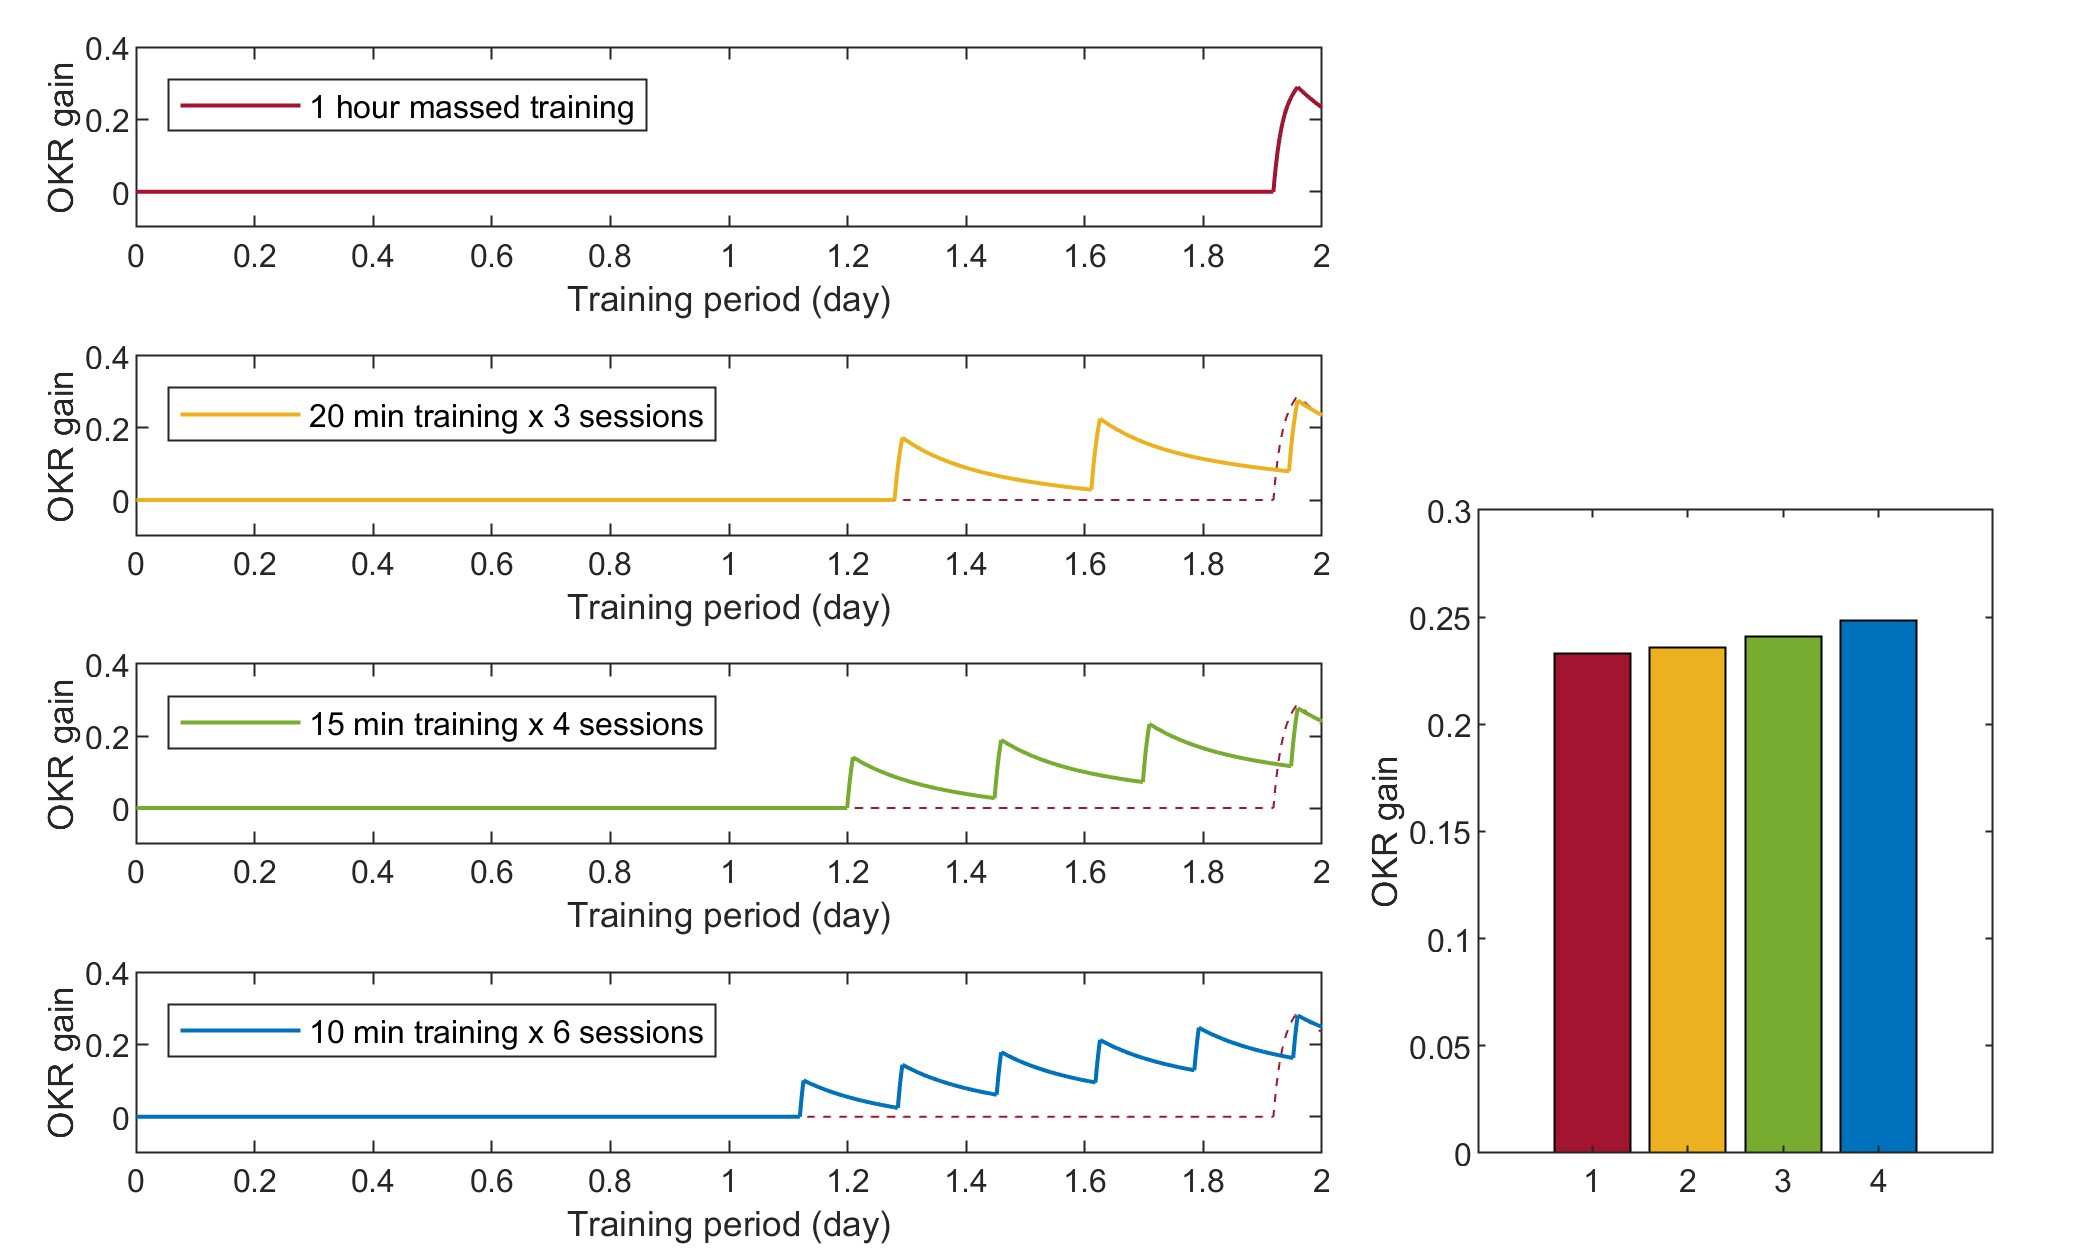
\includegraphics[scale=0.18]{images/training_ltd-deficient.jpg}
    \caption{A comparison between massed vs spaced training for a mouse with genetic deficiencies in spontaneous PF-LTD. The line plots depict OKR gain during the training process. The bar plot compares the values of OKR gain after 1 hour of recovery following the final training session.}
    \label{fig:training_ltd-deficient}
\end{figure}

As was the case when comparing massed vs spaced training in normal mice, the spaced trainings led to an increase in final OKR gain when compared to massed training. However, this time, the improvement is marginal, with only a difference of about 0.02 between the best case (6 sessions of 10 minute training) and the worst case (1 session of 1 hour massed training). While it is not clear at this small scale, by zooming into the line plots in MATLAB, we can actually see that the massed training regime reached a slightly higher peak OKR gain value when compared to any of the spaced alternatives.

\newpage

\subsubsection{Combining Genetic Deficiencies}

Here are the plots of OKR gain and the synaptic weights of the PF-PC and MF-VN synapses from the simulated training of a mouse with both genetic deficiencies in spontaneous PF-LTD and depletion of the GABA receptors in the Purkinje cells.

\begin{figure}[h]
    \centering
    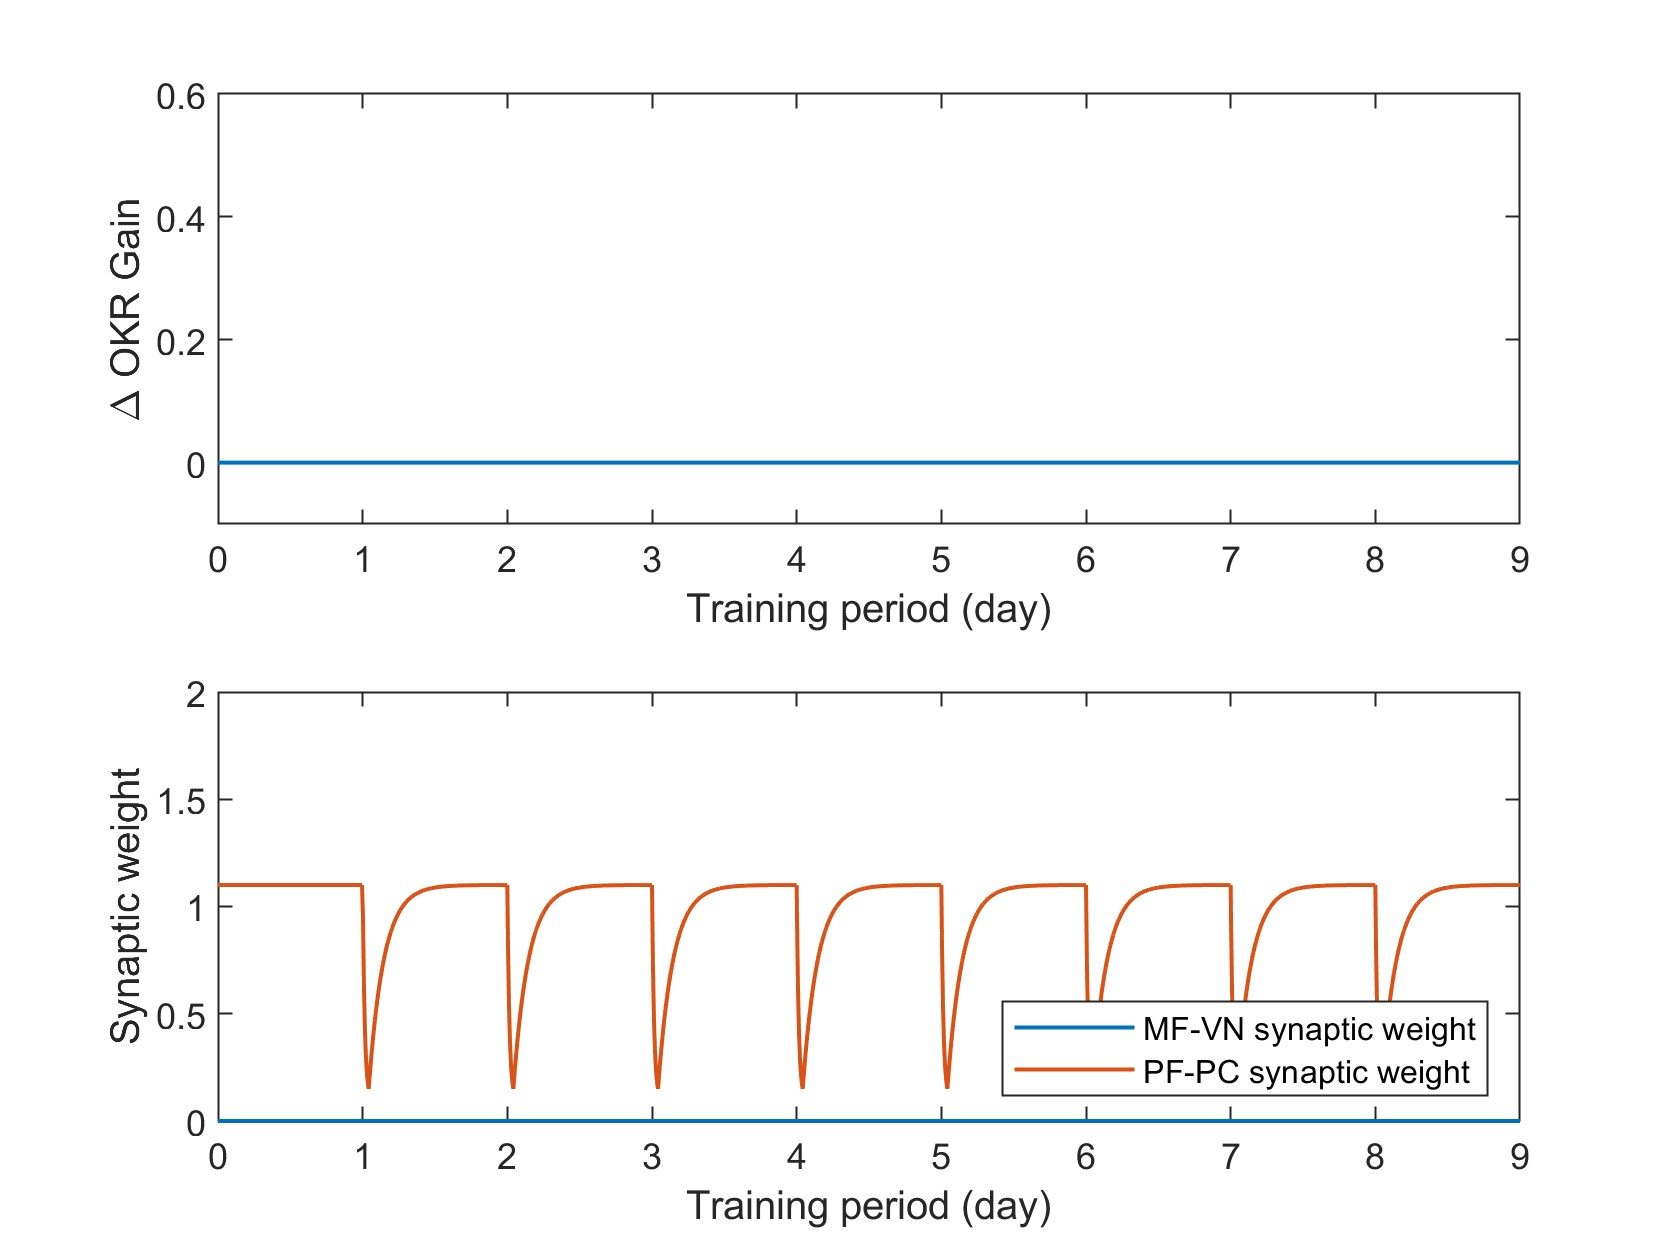
\includegraphics[scale=0.13]{images/combined_LTD-deficiency_GABA-depletion.jpg}
    \caption{Plots of the change in OKR gain and synaptic weights of the PF-PC and MF-VN synapses during training of a mouse with both genetic deficiencies in spontaneous PF-LTD and depletion of GABA receptors in Purkinje cells.}
    \label{fig:combined-gene-results}
\end{figure}

Here we see that the PF-PC synaptic weights change normally during training and recovery, but the MF-VN synaptic weight and change in OKR gain each remain 0.

\section{Discussion and Conclusions}

\subsection{Normal Conditions}

The behavior of the system demonstrated in Figure \ref{fig:normal_okr_adaptation} can be explained by both MF-LTP and PC-LTD. During training, LTD at the PF-PC synapse reduces activation of the Purkinje cells, thereby reducing the inhibition of the vestibular nuclear neurons from the PCs. This increase in VN activity causes LTP at the MF-VN synapses via Hebbian learning. The combined effects of stronger excitation from the mossy fibers and weaker inhibition from the Purkinje cells results in a sharp rise in OKR gain, representing the formation of short term memory during training. Following training, the PF-PC synapse recovers via spontaneous PF-LTD, again inhibiting activation of the VNs. This slows, and eventually stops learning at the MF-VN synapse. During this recovery time, we see a gradual decrease in OKR gain. However, the strengthed MF-VN synapses leaves the vestibular neurons more activated than before learning, so OKR gain does not reduce all the way to its pre-learning levels. This process represents the consolidation of short-term memory into long-term memory during the post-training period. This supports the hypothesis that MF-LTP and PF-LTD are compatible mechanisms for motor learning, rather than needing to be conflicting hypotheses.

\subsection{Massed vs Spaced Training}

Observing the plots of Figure \ref{fig:normal_okr_adaptation}, we can see that the increases in OKR gain slow as training continues. Referring to \eqref{9} and \eqref{12}, this result makes sense: OKR gain is governed by the difference in the synaptic weights of the MF-VN and PF-PC synapses. Spontaneous PF-LTD at the PF-PC synapse is proportional to the current synaptic weight, so as LTD continues its effects are slowed. Thus, the increase in activation of the VNs and LTP at the MF-VN synapses are slowed  as well. With this in mind, we are prepared to analyze Figure \ref{fig:mass_vs_spaced_training}.

Observing the bar plots, we can immediately see that splitting up the hour of training into multiple spaced sessions leads to beneficial increases in OKR gain with the same total training time, as expected from the results of \cite{yamazaki2015modeling} and their real-world motivation we are trying to replicate. This takes advantage of the previous observation that OKR gain increases fastest at the start of training, when the PF-PC synapse is at its baseline level. Of particular interest is the comparison between 4 sessions of 15 minute training separated by 1 hour vs 1 day. When 15 minute training sessions begin on the hour, there is not sufficient recovery time for spontaneous PF-LTD to return the PF-PC synapses to their baseline weight. The short recovery time still yields beneficial results over 1 hour of massed training, but allowing time for full recovery leads to even larger gains.

\subsection{Training Genetically Modified Mice}

The plots in Figure \ref{fig:gene-modified_training} strongly show the distinct roles PF-LTP and PF-LTD play in motor learning of the optokinetic response.

Under the PF-LTP-deficient condition, the synaptic weights of the PF-PC synapses are unable to ever recover, so they have decreased to 0 over time with PF-LTD. Since the synaptic weight has nowhere to decrease during training, increases in OKR gain cannot occur during train. This demonstrates that PF-LTP during post-training recovery time is important for both long-term and short-term memory formation. As explained in the discussion of the simulation under normal conditions, recovery of the PF-PC synapse via PF-LTP plays a role in the consolidation of long-term memory by slowwing Hebbian learning at the MF-VN synapses. However, we can see here that without PF-LTP, short-term learning can occur either. Although short-term learning is caused more directly by PF-LTD, without PF-LTP, the synaptic weight has no room to decrease, and thus PF-LTD cannot form short term memories.

The plot of the PF-LTD deficient case demonstrates the role of PF-LTD in memory formation. Recall that this simulation models only deficiencies in spontaneous PF-LTD, and that PF-LTD is assumed to still occur during training. We can see that short term memories are still formed during training, however long term memories are not consolidated during recovery, with OKR gain continuously decreasing until the next training period begins. Comparing this with the results of Figure \ref{fig:normal_okr_adaptation}, it is clear that spontaneous PF-LTD plays a key role in the consolidation of long-term memory in motor learning.

Finally, we consider the case of selected depletion of GABA receptors in Purkinje cells. In this case, small increases in OKR gain are made during training, but no long-term memories are consolidated during recovery. This makes sense, as the increased activation of the Purkinje cells leaves the vestibular nuclear neurons consistly inhibited. During training, PF-LTD leads to this inhibition giving up just enough for short term improvements in OKR gain, but does not allow for enough activation of the VNs to activate MF-LTP. Thus, as the PF-PC synapse recovers its strength posttraining, OKR gain returns to it's baseline level.

\subsection{Model Extensions}

\subsubsection{The Effect of Time Constants}

Analyzing Figure \ref{fig:time_constants} provides further evidence for the roles of PF-LTD and MF-LTP in motor learning of the optokinetic response. We observed that \(\tau_{learn}\) has a negative relationship with OKR gain. This makes sense because \(\tau_{learn}\) dictates the rate of PF-LTD during training. The faster the synaptic weight is weakened, the less the Purkinje cells are activated and inhibiting the vestibular nuclear neurons and the more MF-LTP and improvements in OKR gain can occur.

We next observed that \(\tau_{recov}\) has a positive relationship with OKR gain, which again makes sense. \(\tau_{recov}\) dictates the rate at which the PF-PC synapses recover during posttraining, so the larger \(\tau_{recov}\) is, the longer these synapses stay weak, and, as with the previous example, the more the VNs are activated.

Finally, we observe that \(\tau_v\) has an inverse relationship with OKR gain. This again makes sense, because a larger \(\tau_v\) means a slower rate of MF-LTP, resulting in lower overall excitation of the VNs and thus lower OKR gain.

\subsubsection{Massed vs. Spaced Training with LTD-Deficiency}

As with the comparison of massed vs spaced training in normal mice, there is a slight increase in performance from shorter, spaced training sessions. The benefits were smaller this time because long term memories are not consolidated in the case of PF-LTD deficiency. Were recovery allowed to continue, OKR gain in all cases would have returned to 0. However, the promising results of the spaced training does suggest that a mouse with deficiency in spontaneous PF-LTD could maintain reasonable OKR gain values with often enough training. These results are consistent with our hypothesis.

\subsubsection{Combining Genetic Deficiencies}

The results in Figure \ref{fig:combined-gene-results} were contrary to our hypothesis. Mice with either deficiencies in PF-LTD or depletion of PC GABA receptors both exhibited short term memory formation during training, but no long-term memory consolidation during recovery. By combining the effects, no short term memories were formed either, contrary to our expectations. However, upon closer reflection, particular by observing the synaptic weights, these results make sense.

In the case of PF-LTD deficiency, short term memories could be formed because inhibition of the PCs from the MLIs allowed the VNs to become active. However, by combining this deficiency with depletion of GABA receptors, the Purkinje cells are never inhibited, thus continuously inhibiting the VNs and never allowing LTP to occur at the MF-VN synapses or adaptation in OKR gain to be exhibited. From a mathematical standpoint, \(v\) is always less than \(w\) in the case of PF-LTD deficiency, however the constant \(w_{MLI}\) allowed the threshold to be past for MF-LTP and short term increases in OKR gain. By setting \(w_{MLI}=0\), the threshold could no longer be satisfied.

This simulation result was particular interesting, because it demonstrated that by combining experimental changes which each individually stopped long-term memory consolidation, we could also stop the formation of short-term memories. The formation of short-term memory is facilitated by the decrease in activation of the Purkinje cells. Two mechanisms by which this occurs is the inhibition from molecular-layer interneurons, via the GABA receptors, and long-term depression at the PF-PC synapses. When either of these mechanisms is deficient, the other can still lessen the activation of the Purkinje cells enough to cell the formation of short term memories. However, with deficiencies in both of these mechanisms, even short term memories cannot be formed.

\section{Statement of Project Contributions}

In coming to understand the model, Daniel focused on the mathematical derivations and Marcelo focused on the underlying physiology, with discussions to help the other understand too.

In recreating the model in MATLAB, Daniel implemented the base model and massed vs spaced training paradigms. Marcelo implemented the simulations for the genetically modified mice.

In extending the model, we swapped areas to round out our understandings. Daniel implemented the extension for combining genetic deficiencies, and Marcelo implemented the extensions for examining the effects of time constants and the effect of training regimes for LTD-deficient mice.

\bibliographystyle{ieeetr}
\bibliography{ref}

\end{document}